\chapter*{LAPORAN}

\section{Perbedaan python 2 dan python 3 }
\par

Python merupakan bahasa pemrograman yang dapat digunakan dengan berbagai paradigma. Mulai dari scripting sederhana hingga object oriented sehingga sangat cocok untuk penggunaan sehari – hari. Python sendiri dipakai diberbagai industri, seperti misalnya industri aeronautica, bahkan studio besar seperti Industrial Light & Magic yang notabene subsidiari dari Lucasfilm (Disney) – penggarap VFX film besar seperti Avenger dan sekuel Star Wars. Sebagian besar industri animasi terlebih pengguna Autodesk Maya memang menggunakan Python untuk membantu pekerjaan. Python menawarkan potensi yang luar biasa.
Seperti yang penulis sampaikan sebelumnya, Pyhton dikembangkan pertama kali oleh Guido van Rossum pada akhir tahun 1980 dan dipublikasikan pertama kali pada 1991. Disebut sebagai penerus pemrograman ABC, Python pada awal rilis sudah disertai dengan fungsi seperti exception, function bahkan class dengan inheritance. Ketika itu sebuah Usernet newsgroup bernama comp.lang.python dibuat di 1994, grup ini membentuk langkah awal untuk Python sebagai salah satu bahasa pemrograman yang sangat populer untuk pengembangan Open Source Software.
Sebelum melihat ke kesempatan yang berkaitan dengan judul yaitu perbedaan mendasar antara Python 2 dan Python 3, mari kita lihat latar belakang rilis major Python.
Python 2
Dipublikasikan pada akhir tahun 2000, Python 2 dinilai lebih transparan dan inklusif untuk pengembangan software ketimbang versi sebelumnya. Hal ini didukung dengan adanya PEP – Python Enhancement Proposal, sebuah spesifikasi teknis yang menjadi tuntunan informasi untuk penggunanya dan menggambarkan fitur baru pada Python itu sendiri.
Sebagai tambahan, Python 2 dilengkapi dengan berbagai fitur programatikal seperti cycle-detecting garbage collector untuk mengotomasi manajemen memori, peningkatan dukungan untuk Unicode, list comprehension untuk membuat sebuah list berdasarkan list yang sudah ada. Unifikasi pada tipe data Python dan class ke satu hirarki terjadi pada rilis Python 2.2
Python 3
Python 3 diharapkan sebagai masa depan Python dan merupakan versi yang saat tulisan ini dibuat masih aktif dikembangkan. Python 3 sendiri adalah versi dengan banyak perubahan yang dirilis akhir tahun 2008. Fokus dari Python 3 itu sendiri adalah untuk melakukan perapian pada codebase dan menghapuskan duplikasi (redundancy). Perubahan terbesar pada Python 3 termasuk memasukkan statemen print ke dalam built-in function.
Awalnya, Python 3 mengalami hambatan pada pengadopsiannya. Itu akibat dari tidak adanya backwards compatibility dengan Python 2. Hal ini membuat pengguna Python sangat berat hati untuk pindah ke versi 3 ini. Tambahannya, banyak sekali library yang hanya tersedia untuk Python 2., tapi setelah tim pengembangan di balik Python 3 telah berulang kali menjelaskan bahwa dukungan terhadap Python 2 akan segera dihentikan, dan semakin banyak libary disalin ke Python 3, maka penerapan Python 3 semakin lama semakin meningkat.
Python 2.7
Dengan dirilisnya Python 3 pada tahun 2008, Python 2.7 dirilis pada Juli 2010 dan direncanakan sebagai rilis 2.x terakhir. Misi dibalik Python 2.7 adalah untuk membuat pengguna Python 2 dengan mudah berpindah ke Python 3 dengan mempersiapkan beberapa kompatibilitas diantara keduanya. Kompatibilitas termasuk peningkatan modul untuk 2.7 seperti unittest untuk mendukung otomasi tes, argparse untuk parsing opsi command-line dan tidak lupa collection dengan class yang lebih baik.
Karena Python 2.7 berada pada posisi yang unik, di antara iterasi Python 2 dan Python 3, maka versi ini menjadi versi yang terbanyak dipergunakan, bahkan jadi versi yang cukup populer untuk dipergunakan dikalangan pengembang. Python 2.7 akan segera dihentikan dukungannya pada tahun 2020.

Cukup sudah bicara sejarah dan overviewnya, mari bicara inti dari artikel kali ini. Perbedaan mendasar antara Python 2 dan Python 3. Meski Python 2.7 dan Python 3 memiliki beberapa kesamaan kapabilitas, namun keduanya tidak sepenuhnya sama.
 
Print
Pada Python2, print diperlakukan seperti statemen ketimbang sebuah function.
1	print “Aku anak Indonesia”
Sedangkan pada Python 3, print diperlakukan sebagai function.
1	print(“Aku anak Indonesia”)
Perubahan ini membuat sintaksis pada Python lebih konsisten. Penggunaan print()  juga kompatibel dengan Python 2.7.
 
Pembagian pada Integer
Pada Python 2, semua tipe data angka yang tidak mengandung desimal akan diperlakukan sebagai integer. Terlihat mudah pada awalnya, ketika mencoba untuk membagi kedua integer akan didapatkan tipe data float.
1	3 / 2 = 1.5
Python 2 menggunakan floor division atau dibulatkan ke nilai paling rendah misalnya 1.5 jadi 1, 2.6 jadi 2 dan seterusnya. Pada Python 2.7 akan menjadi seperti ini
1
2
3
4	x = 3 / 2
print a
#Output
1
Untuk desimal maka tambahkan jadi seperti ini 3.0 / 2.0  untuk mendapatkan hasil 1.5
Pada Python 3, pembagian pada bilangan integer lebih intuitif :
1
2
3
4	a = 3 / 2
print(a)
#Output
1.5
Kita juga masih bisa melakukan 3.0 / 2.0  untuk mendapatkan 1.5 namun untuk mendapatkan floor division maka pada Python 3 gunakan //  :
1
2
3
4	b = 3 // 2
print(b)
#Output
1
Fitur Python 3 ini tidak kompatibel dengan Python 2.7
Dukungan Unicode
Ketika bahasa pemrograman menangani tipe data string (yang mana merupakan sekumpulan karakter), mereka bisa melakukan beberapa cara berbeda sehingga komputer dapat mengubah angka ke huruf dan simbol lain. Python 2 menggunakan alfabet ASCII secara default, sehingga ketika kita mengetik “Halo!”  maka Python 2 menangani string sebagai ASCII. Terbatas pada beberapa ratus karakter, ASCII mungkin bukan pilihan yang fleksibel untuk menangani proses encoding terutama yang non English.
Untuk menggunakan unicode yang lebih luwes, mendukung lebih dari 128,000 karakter maka kita harus mengetik u”Halo!” , dengan tambahan u  di depannya yang mana berarti Unicode.
Python 3 menggunakan Unicode secara default, yang mana menyelamatkan programmer dari tambahan kode lagi, lebih hemat waktu dan mudah untuk diisikan dan ditampilkan. Karena Unicode mendukung berbagai karakter linguistik yang beragam termasuk menampilkan emoji, penggunaan karakter secara default dengan encoding memastikan perangkat mobile didukung oleh program yang kita buat.
Jika kita ingin kode Python 3 kita mendukung Python 2, tambahkan u di depan string.
 
Kelanjutan Pengembangan
Selain perbedaan mendasar antara Python 2 dan Python 3 secara sintatikal, fakta lain adalah Python 2.7 akan dihentikan dukungannya per tahun 2020 dan Python 3 akan terus dikembangkan dengan fitur yang lebih banyak lagi, dan tentu saja yang lebih penting adalah perbaikan dari bug dan performa. Pengembangan saat ini telah mendukung format string secara literal, kustomisasi pembuatan class secara sederhana dan sintaksis yang lebih bersih dan rapi untuk menangani perkalian matriks.
Pengembangan Python 3 akan terus berlangsung, hal ini berarti pengembang perangkat lunak akan dengan nyaman menggunakan Python 3 karena terus didukung oleh komunitas dengan jangka panjang. Tentu saja hal ini meningkatkan kinerja programmer dan kualitas program yang lebih baik.
 
\section{Serjarah pyhton}
Python diciptakan oleh Guido van Rossum pertama kali di  Centrum Wiskunde & Informatica (CWI) di Belanda pada awal tahun 1990-an. Bahasa python terinspirasi dari bahasa pemrograman ABC. Sampai sekarang, Guido masih menjadi penulis utama untuk python, meskipun bersifat open source sehingga ribuan orang juga berkontribusi dalam mengembangkannya.
Di tahun 1995, Guido melanjutkan pembuatan python di Corporation for National Research Initiative (CNRI) di Virginia Amerika, di mana dia merilis beberapa versi dari python.
Pada Mei 2000, Guido dan tim Python pindah ke BeOpen.com dan membentuk tim BeOpen PythonLabs. Di bulan Oktober pada tahun yang sama, tim python pindah ke Digital Creation (sekarang menjadi Perusahaan Zope). Pada tahun 2001, dibentuklah Organisasi Python yaitu Python Software Foundation (PSF). PSF merupakan organisasi nirlaba yang dibuat khusus untuk semua hal yang berkaitan dengan hak intelektual Python. Perusahaan Zope menjadi anggota sponsor dari PSF.
Semua versi python yang dirilis bersifat open source. Dalam sejarahnya, hampir semua rilis python menggunakan lisensi GFL-compatible. Berikut adalah versi mayor dan minor python berikut tanggal rilisnya.
\begin{itemize}
    \item 
\item    Python 1.0 – Januari 1994
\item	 Python 1.2 – 10 April 1995
\item    Python 1.3 – 12 Oktober 1995
\item    Python 1.4 – 25 Oktober 1996
\item 	 Python 1.5 – 31 Desember 1997
\item    Python 1.6 – 5 September 2000
\item  	 Python 2.0 – 16 Oktober 2000
\item 	 Python 2.1 – 17 April 2001
\item 	 Python 2.2 – 21 Desember 2001
\item  	 Python 2.3 – 29 Juli 2003
\item 	 Python 2.4 – 30 Nopember 2004
\item 	 Python 2.5 – 19 September 2006
\item 	 Python 2.6 – 1 Oktober 2008
\item    Python 2.7 – 3 Juli 2010
\item 	 Python 3.0 – 3 Desember 2008
\item 	 Python 3.1 – 27 Juni 2009
\item 	 Python 3.2 – 20 Februari 2011
\item 	 Python 3.3 – 29 September 2012
\item 	 Python 3.4 – 16 Maret 2014
\item 	 Python 3.5 – 13 September 2015
\item 	 Python 3.6 – 23 Desember 2016
\item 	 Python 3.7 – 27 Juni 2018
\item	 Python 1.0 – Januari 1994
\item	 Python 1.2 – 10 April 1995
\item	 Python 1.3 – 12 Oktober 1995
\item	 Python 1.4 – 25 Oktober 1996
\item	 Python 1.5 – 31 Desember 1997
\item	 Python 1.6 – 5 September 2000
\item	 Python 2.0 – 16 Oktober 2000
\item	 Python 2.1 – 17 April 2001
\item	 Python 2.2 – 21 Desember 2001
\item	 Python 2.3 – 29 Juli 2003
\item  	 Python 2.4 – 30 Nopember 2004
\item    Python 2.5 – 19 September 2006
\item	 Python 2.6 – 1 Oktober 2008
\item	 Python 2.7 – 3 Juli 2010
\item	 Python 3.0 – 3 Desember 2008
\item	 Python 3.1 – 27 Juni 2009
\item	 Python 3.2 – 20 Februari 2011
\item	 Python 3.3 – 29 September 2012
\item	 Python 3.4 – 16 Maret 2014
\item	 Python 3.5 – 13 September 2015
\item	 Python 3.6 – 23 Desember 2016
\item	 Python 3.7 – 27 Juni 2018
\end{itemize}
Nama python sendiri tidak berasal dari nama ular yang kita kenal. Guido adalah penggemar grup komedi Inggris bernama Monty Python. Ia kemudian menamai bahasa ciptaannya dengan nama Python.


\section{5 perusahan penguna pyhton}
\begin{enumerate}
    \item Spotify
Penyedia layanan musik streaming Spotify memanfaatkan Python untuk analisis data dan backend. Pada backend Spotify banyak terdapat service yang berkomunikasi lewat 0MQ (ZeroMQ) yang merupakan framework dan library open source untuk networking. 0MQ dibuat menggunakan Python dan C++. Alasan service dibuat menggunakan Python dikarenakan Spotify sangat menyukai kecepatan pipeline development.
Sistem rekomendasi Spotify bergantung pada analisis data yang sangat besar, untuk menginterpretasikan analisis tersebut Spotify menggunakan Luigi, modul Python yang sinkron dengan Hadoop. Modul open source ini menangani satu library dengan library lainnya agar saling bekerjasama, dan mengkonsolidasi eror log secara cepat.

    \item Google
Dari awal berdiri, Google sudah menggunakan Python, bahkan Python merupakan salah satu bahasa pemrograman yang penting bagi Google, itulah mengapa Google pernah merekrut kreator Python Guido Van Rossum untuk bekerja di Google.
Sebuah kutipan dari pendiri Google “Python where we can, C++ where we must,” kutipan ini artinya jika menginginkan kontrol akan memori dan latensi yang rendah maka gunakan C++, sisanya gunakan Python sebisa mungkin, meskipun ada script yang ditulis untuk Google dalam bahasa Perl atau Bash, nantinya script tersebut akan diubah lagi ke Python, alasannya adalah karena kemudahan dalam perawatan.
Saat ini Python merupakan salah satu bahasa pemrograman server-side resmi di Google, selain Pyhton Google juga menggunakan C++, Java dan Go

    \item Industrial Light and Magic
ILM adalah Studio spesial-efek yang didirikan oleh George Lucas pada tahun 1975, awalnya studio ini membuat berbagai efek yang dibutuhkan untuk film Star Wars saja, namun studio ini berkembang pesat dan meraih banyak penghargaan. Seiring berkembangnya teknologi komputer , ILM meyakini bahwa CGI merupakan masa depan bagi efek visual dan mulai mencari sistem yang tepat. Karena infrastruktur awal ILM dibuat menggunakan C dan C++, maka akan lebih mudah mengintegrasikan Python ketimbang Perl ataupun Tcl. Menggunakan Python, ILM dapat dengan mudah membungkus komponen software dan meningkatkan aplikasi grafis mereka. Hingga saat ini ILM tetap menggunakan Python karena selalu dapat menghadirkan solusi terbaik untuk kebutuhan mereka. 

    \item Netflix
Salah satu penggunaan utama Python di aplikasi Netflix adalah pada Central Alert Gateway. Aplikasi RESTful ini akan me-reroute alert dan mengirimkannya pada kelompok atau individu yang berhak melihatnya. Sebagai tambahan aplikasi ini akan secara otomatis reboot atau menghentikan proses yang dianggap bermasalah. Selain C.A.G, Python juga digunakan pada aplikasi untuk menelusuri riwayat dan perubahan pengaturan keamanan.

    \item Instagram
Seperti yang kita ketahui, Instagram telah merevolusi komunikasi visual dan pemasaran digital melalui media foto. Dengan 400 juta pengguna aktif setiap harinya, tentu ini menghapus pendapat yang mengatakan bahwa aplikasi python tidak terlalu scalable. Menurut Hui Ding, engineer di Instagram, moto para pengembang aplikasi di instagram adalah “Do the simple thing first,” dan hal ini sangat bisa dilakukan menggunakan Python, bagi para pengembang aplikasi di Instagram Python sangat ramah pengguna, sederhana dan rapi. Juga karena Python sangat populer, maka tidaklah sulit menemukan pengembang baru untuk memperbesar tim.


\end{enumerate}
\section{CARA INSTALLER ANACONDA}
\begin{enumerate}
\item 	Pertama buka anaconda pada google, kemudian cari installer anaconda versi 3
\begin{figure}[h]
    \centering
    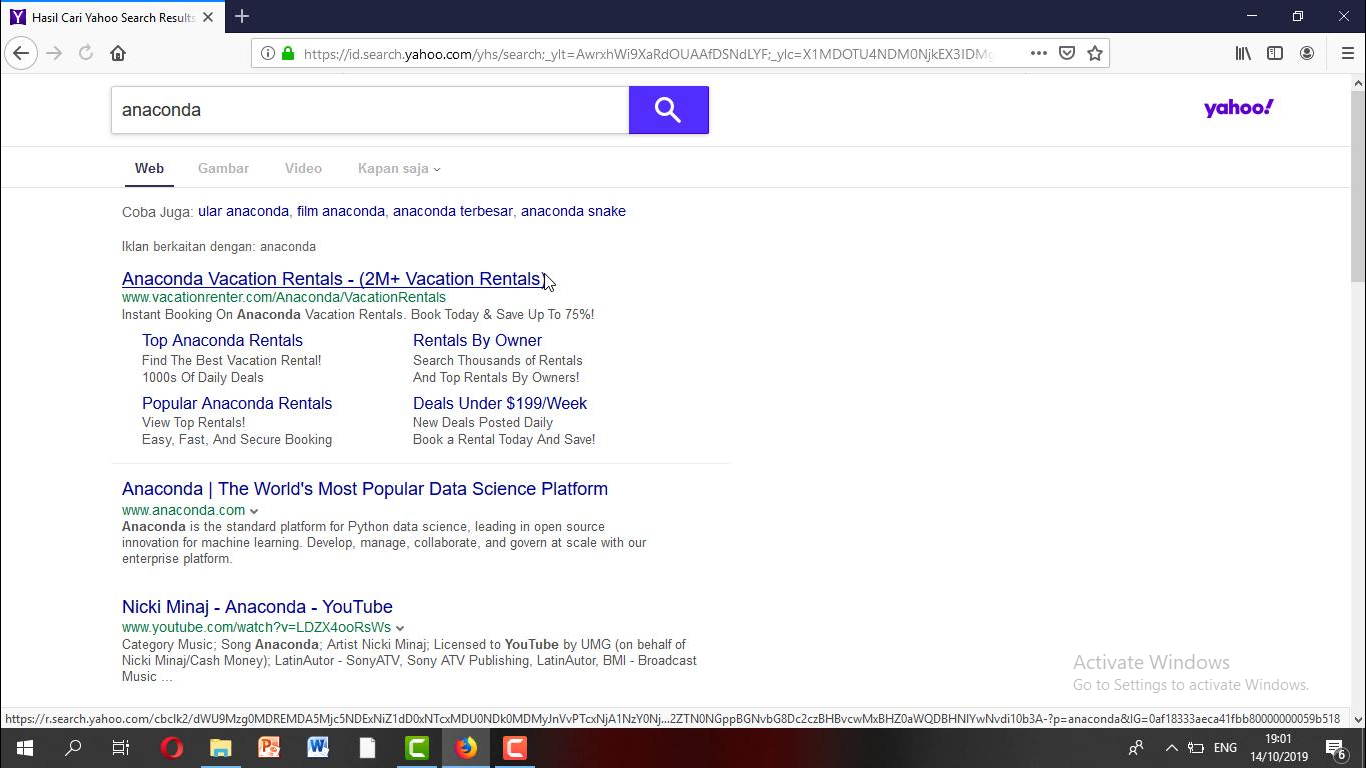
\includegraphics[scale=0.2]{gambar/cara1.png}
    \caption{Gambar1}
    \label{fig:my_label}
\end{figure}
\item Selanjutnya klik download pada pojok kanan atas
\begin{figure}[h]
    \centering
    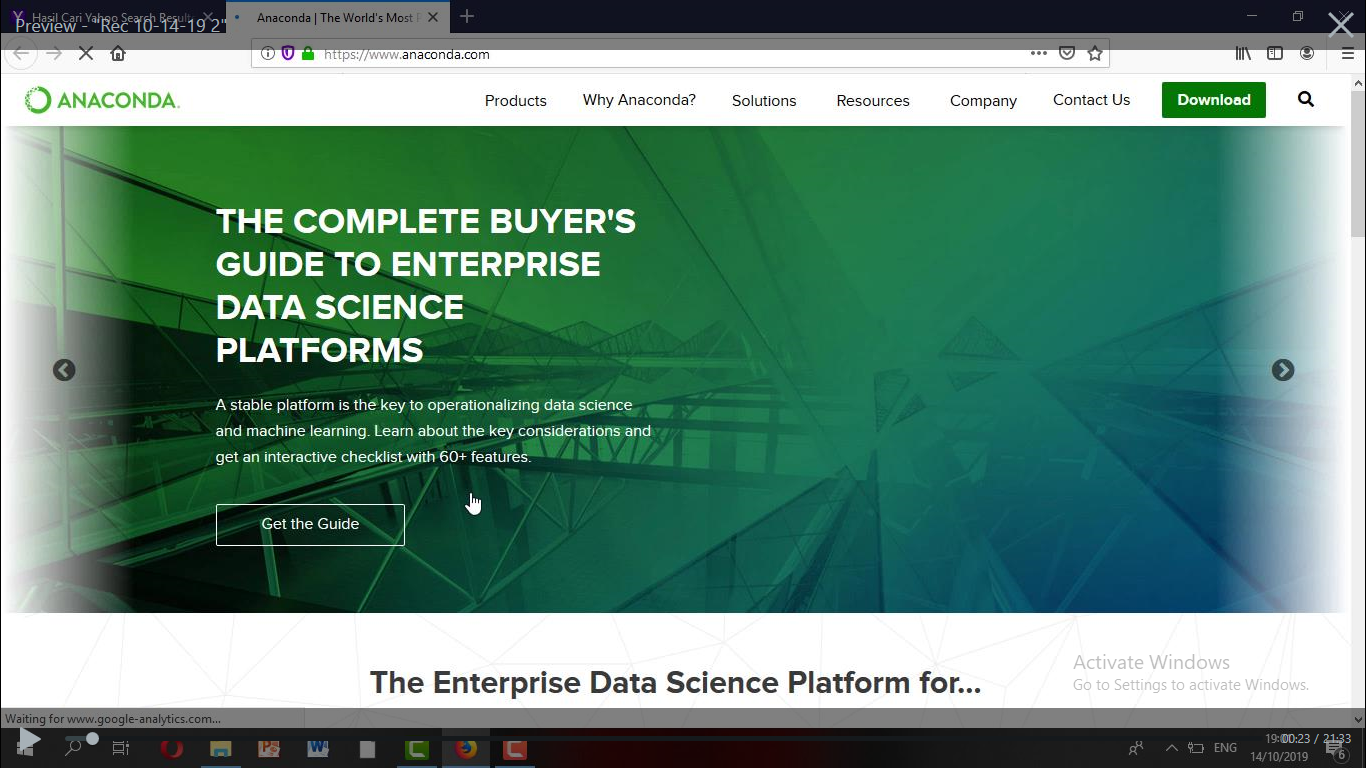
\includegraphics[scale=0.2]{gambar/cara2.png}
    \caption{Gambar2}
    \label{fig:my_label}
\end{figure}
\item Lalu pilih versi tergantung berapa bit laptop anda, kalau laptop anda 32 bit maka pakai yang 32 bit tapi jika laptop anda 64 bit maka pakailah yang 64 bit.
\begin{figure}[h]
    \centering
    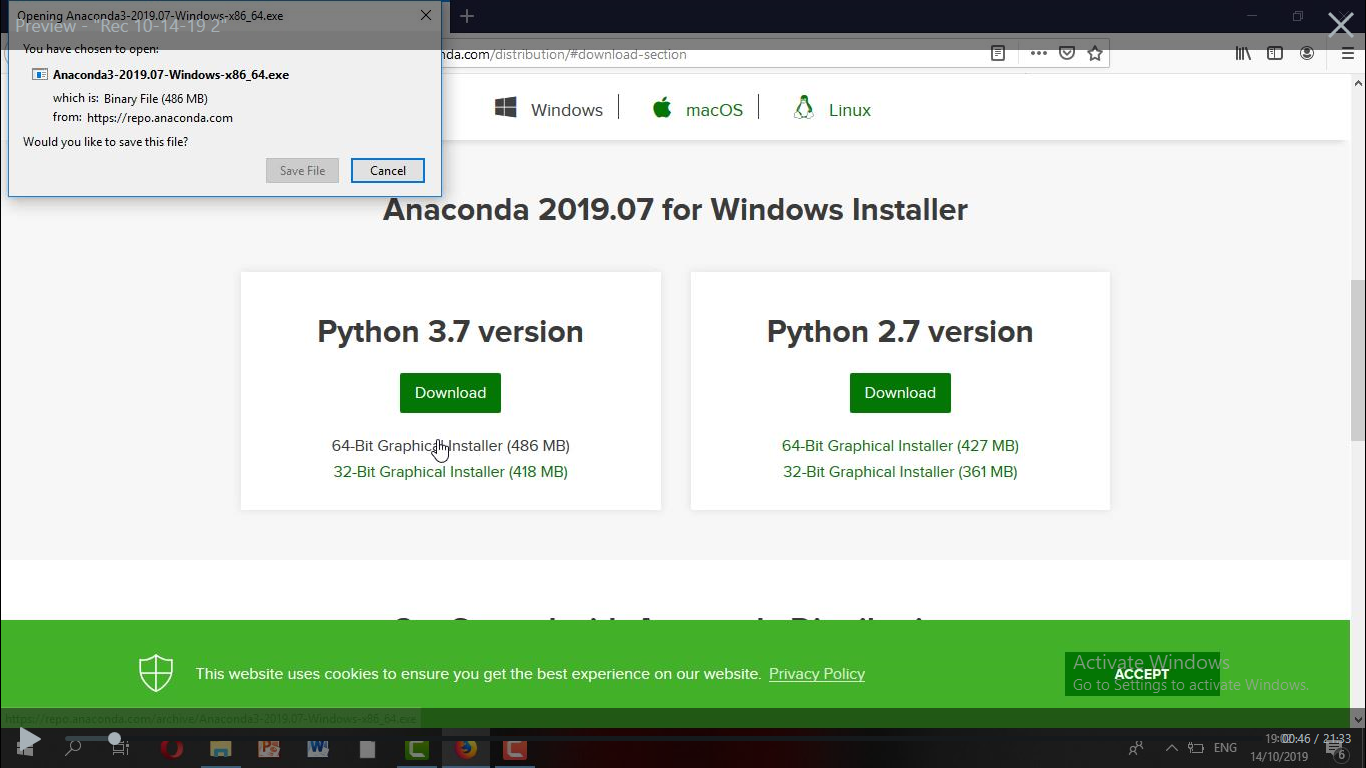
\includegraphics[scale=0.2]{gambar/cara3.png}
    \caption{Gambar3}
    \label{fig:my_label}
\end{figure}
\item	Selanjutnya klik I agree
\begin{figure}[h]
    \centering
    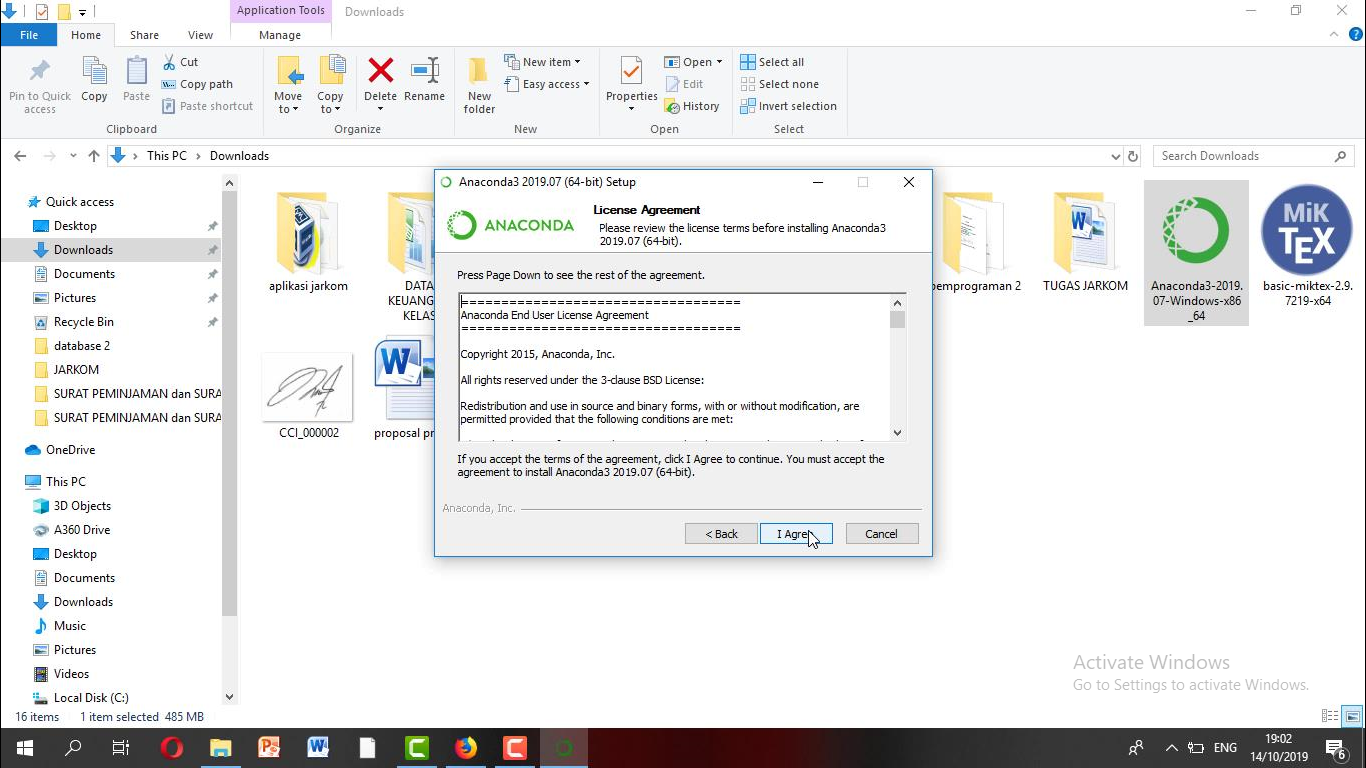
\includegraphics[scale=0.2]{gambar/cara4.png}
    \caption{Gambar4}
    \label{fig:my_label}
\end{figure}

\item Lalu klik next
\begin{figure}[h]
    \centering
    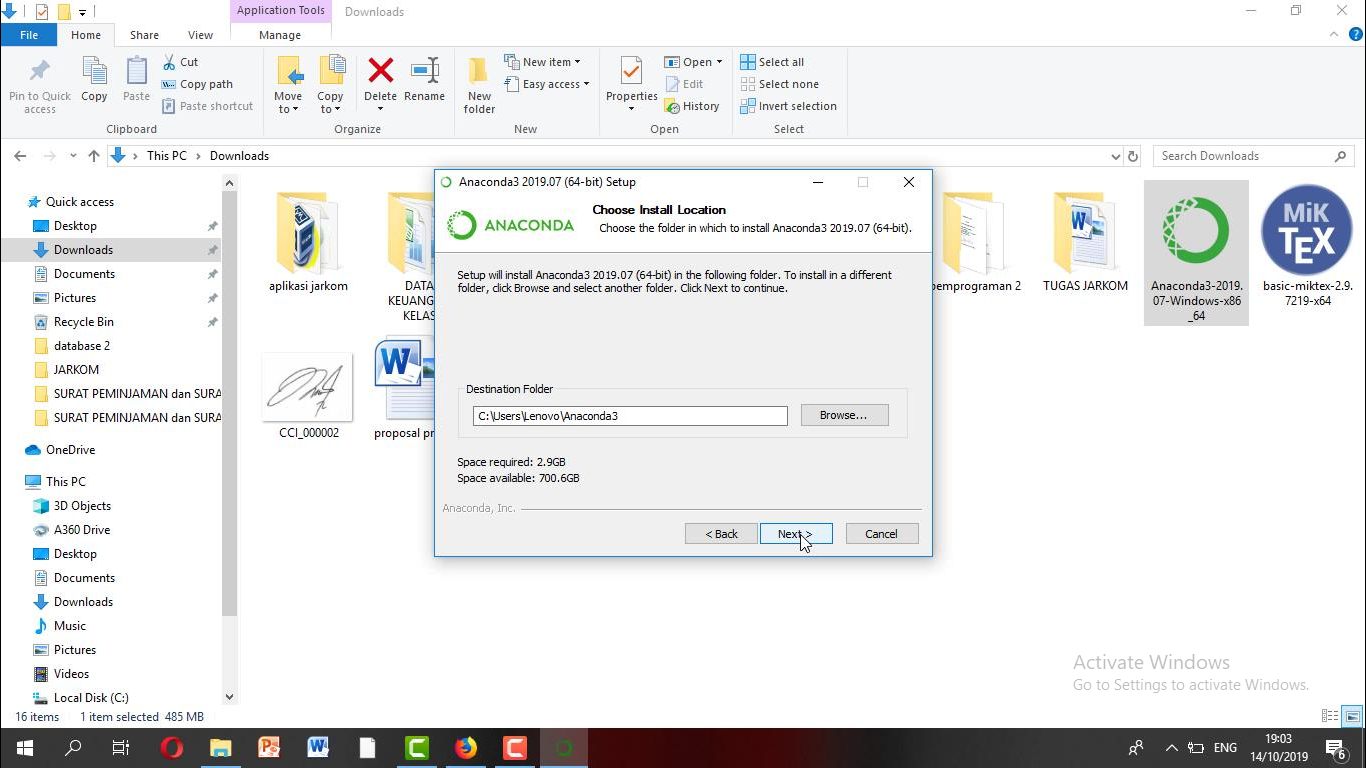
\includegraphics[scale=0.2]{gambar/cara5.png}
    \caption{Gambar5}
    \label{fig:my_label}
\end{figure}
\item Kemudian akan mucul kotak dialog dan centang kedua-duanya, lalu klik install
\begin{figure}[h]
    \centering
    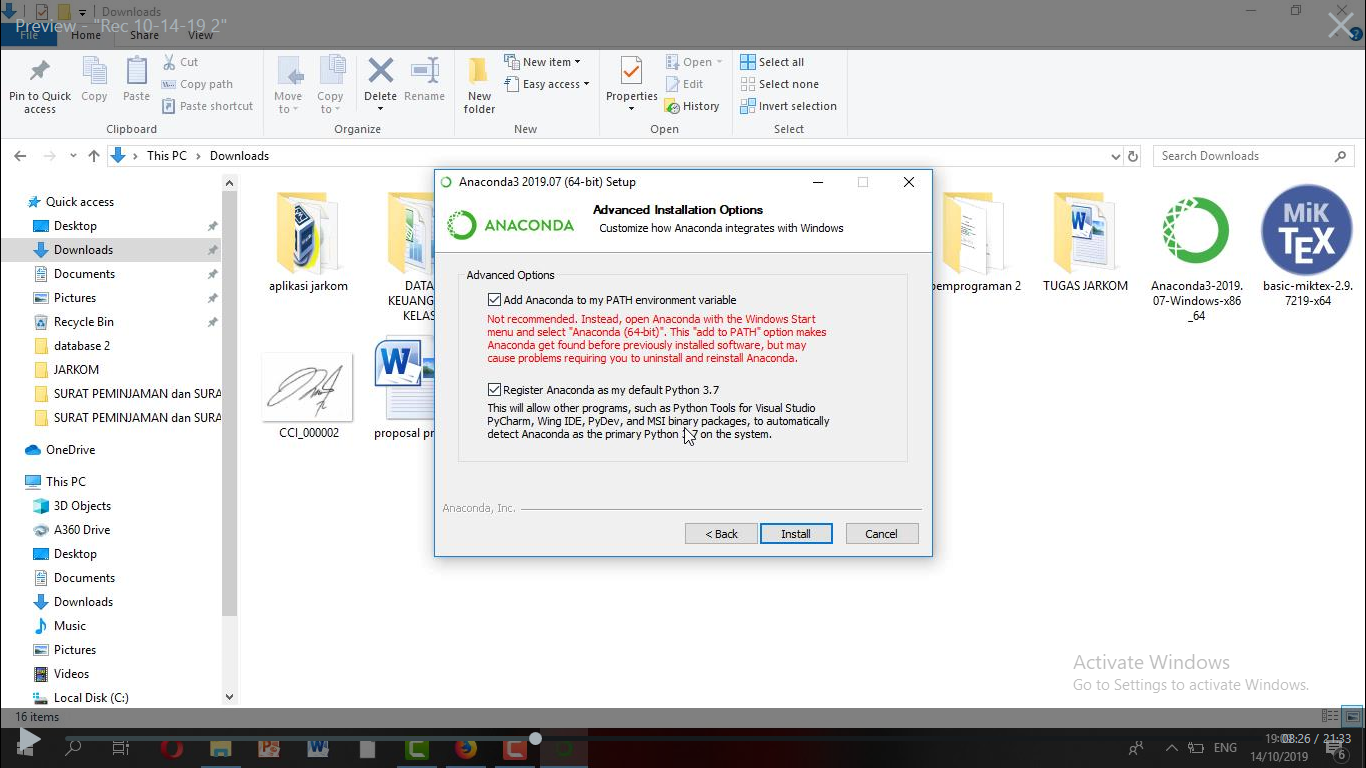
\includegraphics[scale=0.2]{gambar/cara6.png}
    \caption{Gambar6}
    \label{fig:my_label}
\end{figure}
\item Tunggu hingga proses install selesai
\begin{figure}[h]
    \centering
    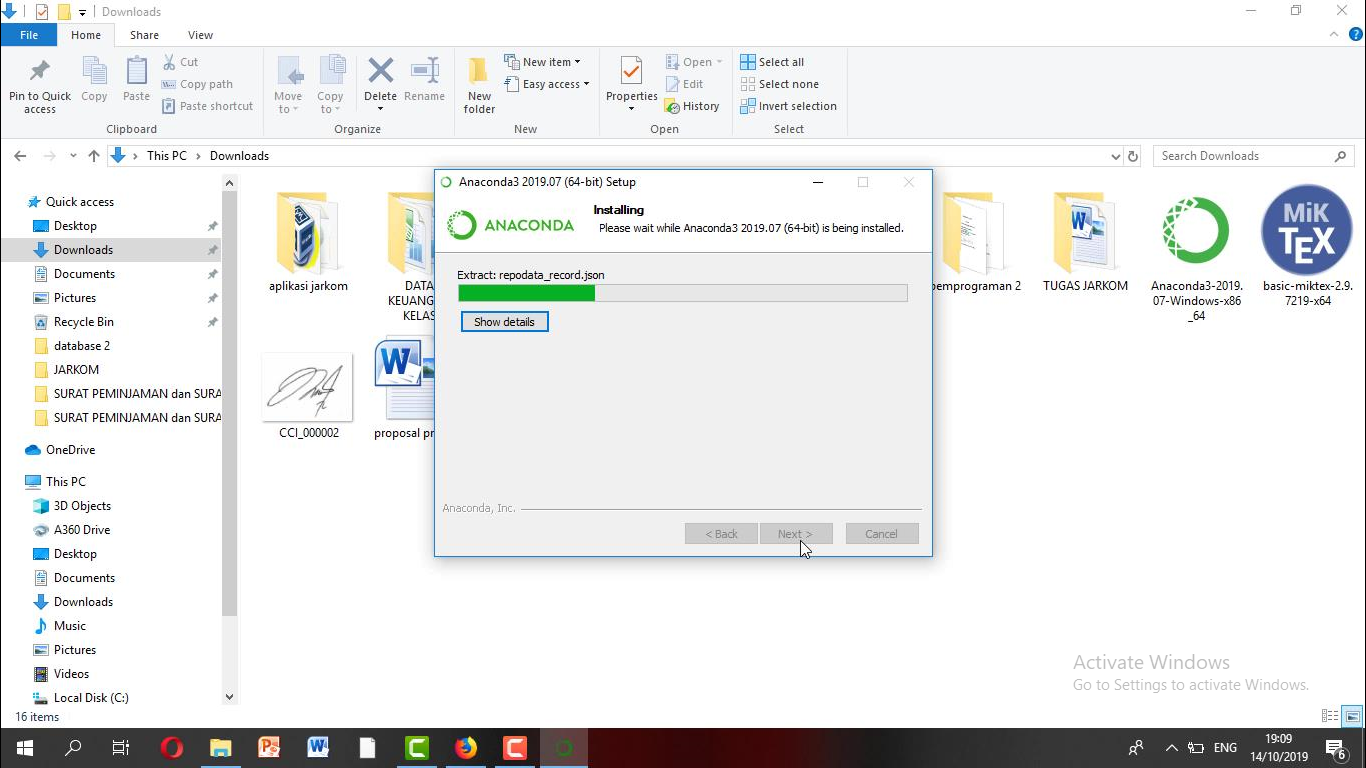
\includegraphics[scale=0.2]{gambar/cara7.png}
    \caption{Gambar7}
    \label{fig:my_label}
\end{figure}
\item Setelah itu klik next
\begin{figure}[h]
    \centering
    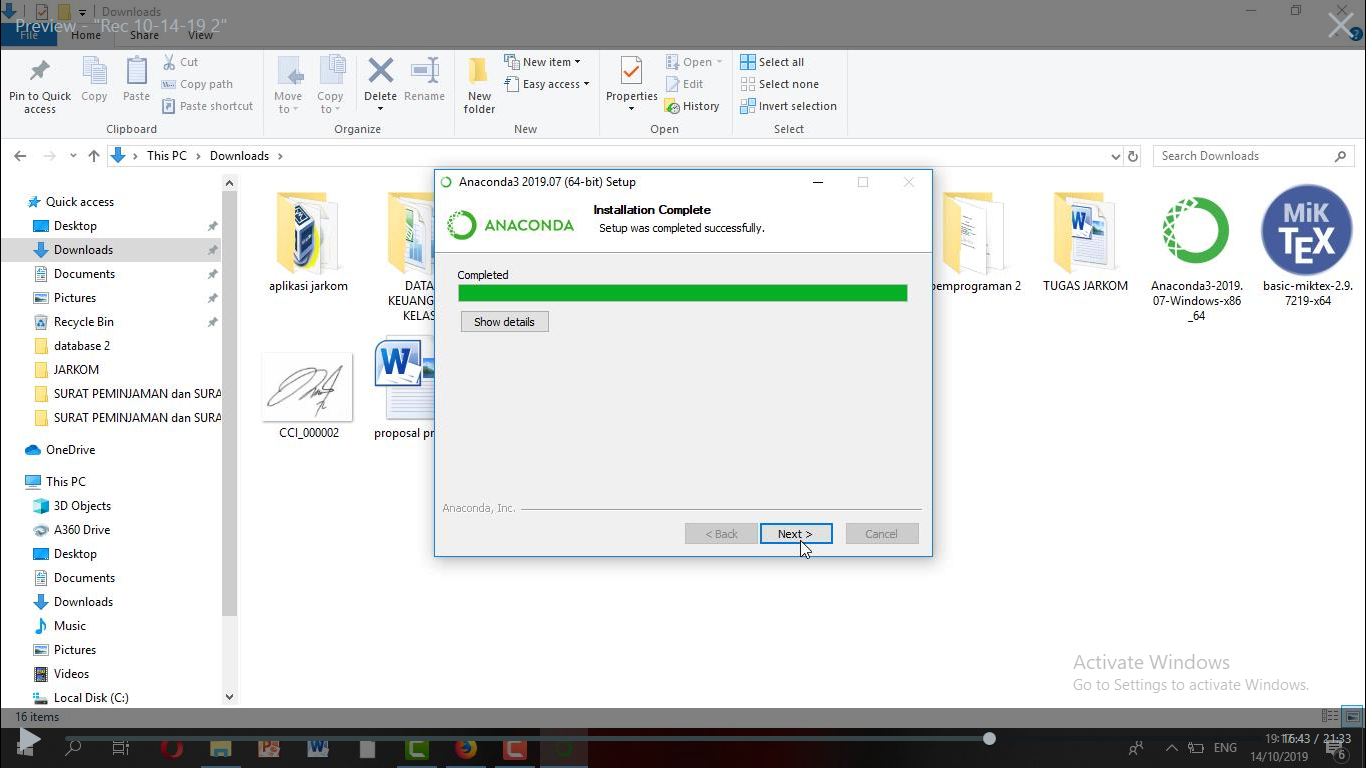
\includegraphics[scale=0.2]{gambar/cara8.png}
    \caption{Gambar8}
    \label{fig:my_label}
\end{figure}
\item Kemudian klik next lagi
\begin{figure}[h]
    \centering
    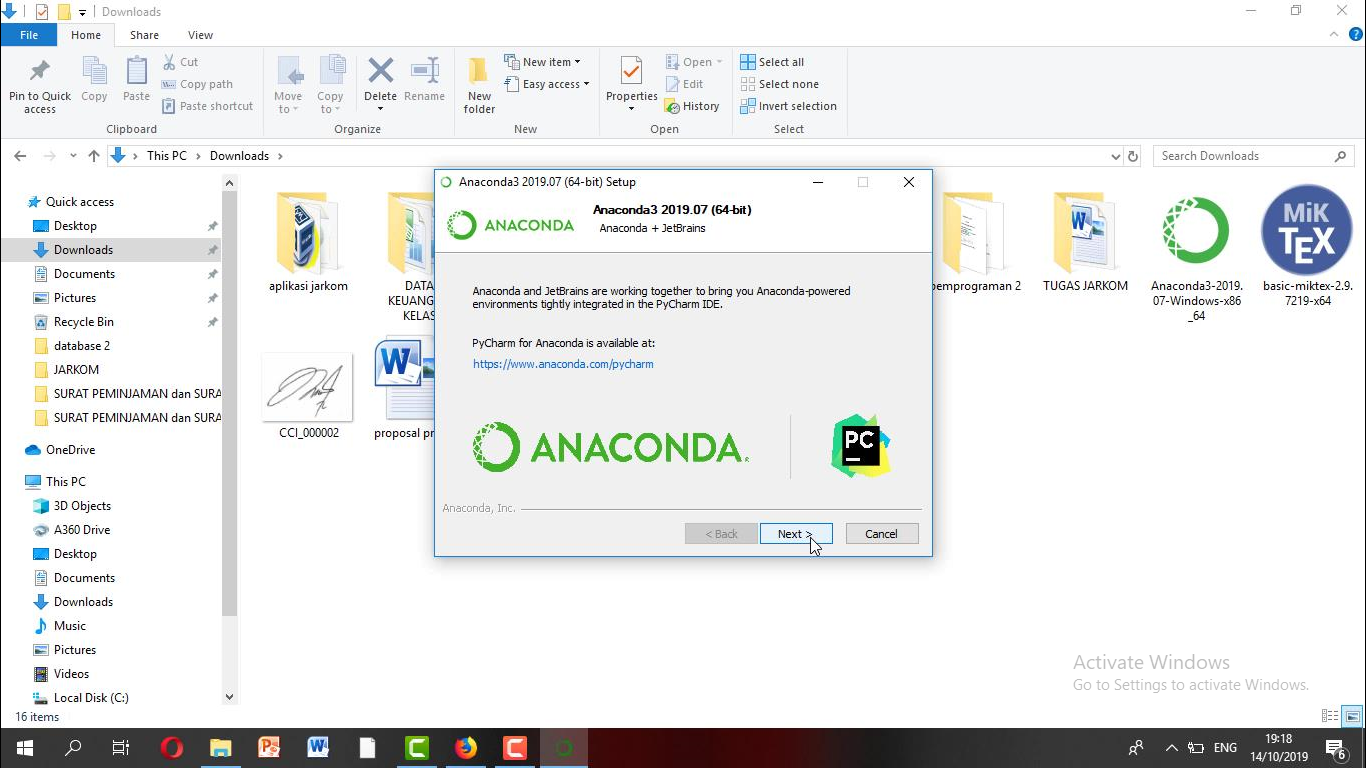
\includegraphics[scale=0.2]{gambar/cara9.png}
    \caption{Gambar9}
    \label{fig:my_label}
\end{figure}
\item Dan klik finis
\begin{figure}[h]
    \centering
    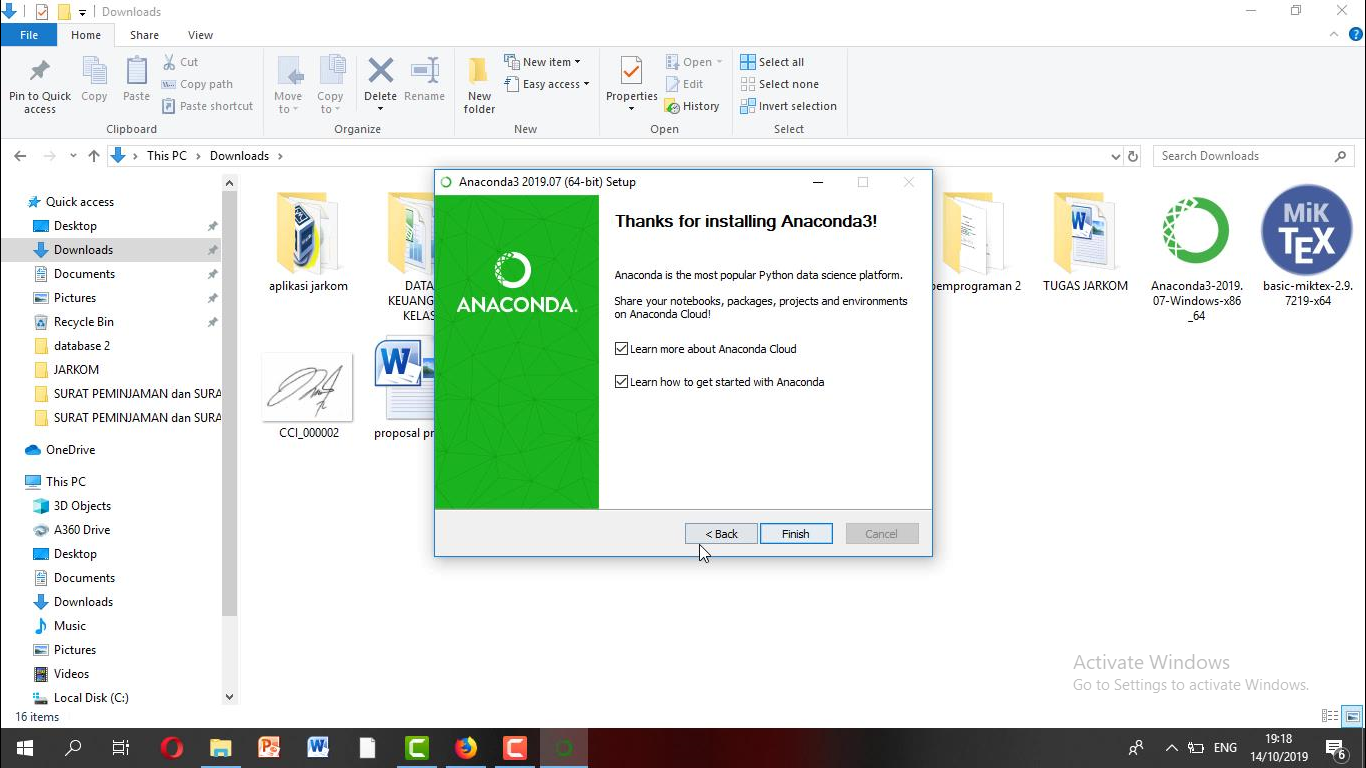
\includegraphics[scale=0.2]{gambar/cara11.png}
    \caption{Gambar10}
    \label{fig:my_label}
\end{figure}
\end{enumerate}